\documentclass{bioinfo}
\copyrightyear{2019}
\pubyear{2019}

\usepackage{natbib}
\bibliographystyle{apalike}

\begin{document}
\firstpage{1}

\title{Identifying centromeric satellites with dna-brnn}
\author[Li]{Heng Li$^{1,2,3}$}
\address{$^1$ Department of data sciences, Dana-Farber Cancer Institute, 450 Brookline Ave, Boston, MA 02115, USA\\
$^2$ Department of biomedical informatics, Harvard Medical School, 25 Shattuck Street, Boston, MA 02115, USA\\
$^3$ Broad Institute, 415 Main St, Cambridge, MA 02142, USA}

\maketitle

\begin{abstract}

\section{Summary:} Human alpha satellite and satellite 2/3 contribute to
several percent of the human genome. However, identifying these sequences with
traditional algorithms is computationally intensive. Here we develop dna-brnn,
a recurrent neural network to learn the sequences of the two classes of
centromeric repeats. It achieves high similarity to RepeatMasker and is tens of
times faster. Dna-brnn explores a novel application of deep learning and may
accelerate the study of the evolution of the two repeat classes.

\section{Availability and implementation:}
\href{https://github.com/lh3/dna-nn}{https://github.com/lh3/dna-nn}

\section{Contact:} hli@jimmy.harvard.edu
\end{abstract}

\section{Introduction}

Eukaryotic centromeres consist of huge arrays of tandem repeats, termed
\emph{satellite DNA}~\citep{Garrido-Ramos:2017aa}. In human, the two largest
classes of centromeric satellites are alpha satellite (alphoid) with a 171bp
repeat unit, and satellite II/III (hsat2,3) composed of diverse variations of
the ${\tt ATTCC}$ motif. They are totaled a couple of hundred megabases in
length~\citep{Schneider:2017aa}. Both alphoid and hsat2,3 can be identified
with RepeatMasker~\citep{Tarailo-Graovac:2009aa}. However, RepeatMasker is
inefficient. Annotating a human long-read assembly may take several days using
32 CPUs; annotating high-coverage sequence reads is practically infeasible. In addition, RepeatMasker requires RepBase~\citep{Kapitonov:2008aa},
which is not commercially free. In practice, we do not often apply RepeatMasker
to human assemblies.

We reduce repeat annotation to a classification problem and solve the problem
with a neural network. Because the repeat units of alphoid and hsat2,3 are
short, we can learn their sequences with a small network and achieve high
performance.

\begin{methods}
\section{Methods}

\subsection{The dna-brnn model}

Given $m$ types of non-overlapping features on a DNA sequence, we can label
each base with number $0,\ldots,m$, where `0' stands for a null-feature.
\mbox{Dna-brnn} learns how to label a DNA sequence. Its overall architecture
(Fig.~\ref{fig:model}) is similar to an ordinary bidirected neural network
(BRNN), except that \mbox{dna-brnn} feeds the reverse complement sequence to the
opposite GRU array and that it ties the weights in both directions. Dna-brnn is
strand symmetric in that the network output is the same regardless of the input
DNA strand. Strand symmetry is not just a nice theoretical property. Without
weight sharing between the two strands, we will end up with a model with twice
as many parameters but 16\% worse training cost (averaged in 10 runs).

In theory, we can directly apply dna-brnn to arbitrarily long sequences.
However, given a single sequence or multiple sequences of variable lengths, it
is non-trivial to implement advanced parallelization techniques and without
parallelization, the practical performance would be tens of times slower. As a
tradeoff, we apply dna-brnn to 150bp subsequences and discard information in a
longer range.

To identify satellites, we assign label `1' to hsat2,3 and label `2' to
alphoid. The size of the GRU hidden vector is 32. There are $<$5000 free
parameters in such a model.

\begin{figure}[tb]
\centering
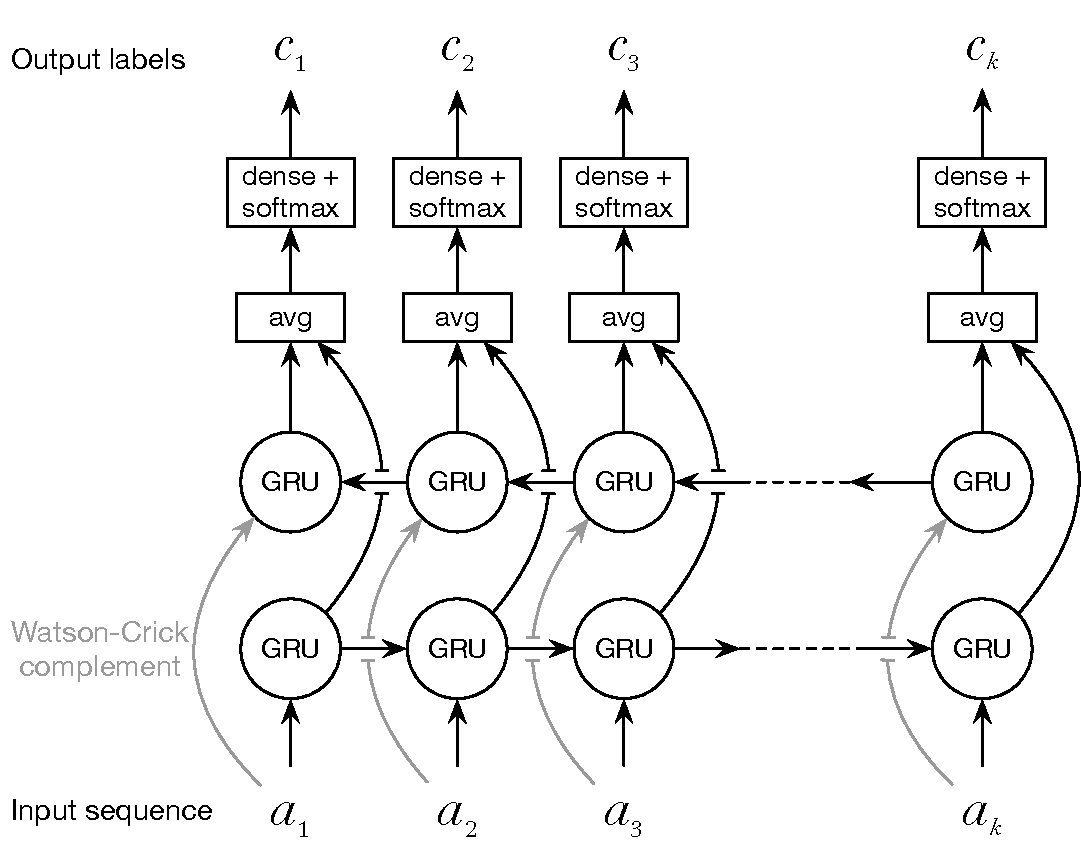
\includegraphics[width=.45\textwidth]{dna-nn-fig}
\caption{The dna-brnn model. Dna-brnn takes a $k$-long one-hot encoded DNA
sequence as input. It feeds the input and its reverse complement to two arrays
of gated recurrent units (GRUs) running in the opposite directions. At each
position, dna-brnn averages the two GRU output vectors, transforms the
dimension of the average with a dense layer and applies softmax. The final
output is the predicted distribution of labels for each input base. All GRUs in
both directions share the same weights.}\label{fig:model}
\end{figure}

\subsection{Training and prediction}

In training, we randomly sample 256 subsequences of 150bp in length and update
the model weights with RMSprop on this minibatch. To reduce overfitting, we
randomly drop out 25\% elements in the hidden vectors. We terminate
training after processing 250Mb randomly sampled bases.

On prediction, we run the model in each 150bp long sliding window with 50bp
overlap. In each window, the label with the highest probability is taken as the
preliminary prediction. In an overlap between two adjacent windows, the label
with higher probability is taken as the prediction. Such a prediction
algorithm works well in long arrays of satellites. However, it occasionally
identifies satellites of a few bases when there is competing evidence. To
address this issue, we propose a post-processing step.

With the previous algorithm, we can predict label $c_i$ and its
probability $p_i$ at each sequence position $i$. We
introduce a score $s_i$ which is computed as
\begin{equation}\label{eq:sc}
t_i=\log\frac{\min(p_i,0.99)}{1-\min(p_i,0.99)},\,\,\,
s_i=\left\{\begin{array}{ll}
t_i & (c_i>0) \\
-10t_i & (c_i=0)\\
\end{array}\right.
\end{equation}
Here $s_i$ is usually positive at a predicted satellite base and negative at a
non-satellite base. Let $S_{a,b}=\sum_{i=a}^b s_i$
be the sum of scores over segment $[a,b]$. Intuitively, we say $[a,b]$ is
maximal if it cannot be lengthened or shortened without reducing $S_{a,b}$.
\citet{DBLP:conf/ismb/RuzzoT99} gave a rigorous definition of maximal scoring
segment (MSS) and a linear algorithm to find all of them. By default,
dna-brnn takes an MSS longer than 50bp as a satellite segment. The use of MSS
effectively clusters fragmented satellite predictions and improves the accuracy
in practice.

\subsection{Training and testing data}

The training data come from three sources: chromosome 11, annotated
alphoids in the reference genome and decoy sequences, all for GRCh37.
RepeatMasker annotations on GRCh37 were acquired from the UCSC Genome Browser.
Repeats on the GRCh37 decoy were obtained by us with RepeatMasker (v4.0.8,
using rmblast-2.6.0+ as the alignment engine). RepeatMasker may annotate
hsat2,3 as `HSATII', `(ATTCC)n', `(GGAAT)n', `(ATTCCATTCC)n' or other rotations
of the ATTCC motif. We combined all such repeats into hsat2,3.  We take the
RepeatMasker labeling as the ground truth.

We use the training data to learn weights in the model. We
annotated GRCh38 decoy sequences~\citep{Mallick:2016aa} with RepeatMasker and used that to tune
hyperparameters, such as the size of GRU and non-model parameters in
Eq.~(\ref{eq:sc}). For testing, we randomly sampled 326Mb sequences from a
CHM1 assembly (AC:GCA\_001297185.1) and annotated them with RepeatMasker as
well. Testing data do not overlap training or validation data.

\subsection{Implementation}

Unlike the majority of deep learning based tools which are written in Python
and depend on heavy framework such as TensorFlow, dna-brnn is implemented in C,
on top of the lightweight KANN framework that we developed. KANN uses CPU only, supports
parallelization and has no external dependencies. This makes dna-brnn easily
deployed without requiring special hardware or software settings.

We have also implemented dna-cnn, a strand-symmetric convolutional neural network
for a similar task. It predicts the fraction of each repeat class on a
fixed-length sequence. Dna-cnn is faster than dna-brnn and can also achieve
high similarity to RepeatMasker. We focus on dna-brnn here because it outputs
per-base annotation.

\end{methods}

\section{Results}

Training dna-brnn takes 6.7 wall-clock minutes using 16 CPUs. Predicting labels
on testing data takes 6.2 minutes.
With rmblast as the alignment engine, RepeatMasker annotates the testing data in
641 minutes using 32 CPUs, 100 times slower. Table~1 shows the testing accuracy
with different prediction strategies. Applying MSS clustering improves both FNR
and FPR. We use the `mss:Y, minLen:50' setting in the rest of the Results
section.

On the testing data, dnr-brnn predicts 70kb hsat2,3 satellites not annotated
by RepeatMasker. We looked at them by eye and had the impression that most of
them are divergent copies of (AATTC)n. Some of them are annotated as other
types of tandem repeats; some are missed. The hsat2,3 FPR of dna-brnn should be
lower considering that the RepeatMasker annotation may be incomplete.

\begin{table}[tb]
\processtable{Evaluation of dna-brnn accuracy}
{\footnotesize
\begin{tabular}{p{3.3cm}rlrl}
\toprule\\[-1.5em]
& \multicolumn{2}{c}{\vspace{0.3em}alphoid} & \multicolumn{2}{c}{hsat2,3} \\
\cline{2-5}\\[-0.7em]
Setting & \multicolumn{1}{c}{FNR} & \multicolumn{1}{c}{FPR} & \multicolumn{1}{c}{FNR} & \multicolumn{1}{c}{FPR} \\[-0.5em]
\midrule
mss:N, minLen:0 & 0.51\% & 1 / 9719  & 0.18\% & 1 / 3954 \\
mss:N, minLen:50& 0.73\% & 1 / 28035 & 0.29\% & 1 / 4575 \\
mss:Y, minLen:50& 0.39\% & 1 / 38020 & 0.17\% & 1 / 4355 \\
mss:Y, minLen:200&0.42\% & 1 / 52240 & 0.39\% & 1 / 6354 \\
mss:Y, minLen:500&0.58\% & 1 / 64335 & 0.65\% & 1 / 13573 \\
\botrule
\end{tabular}
}{RepeatMasker annotations on 326Mb sequences randomly sample from the human
CHM1 assembly are taken as the ground truth. `mss': whether to cluster
predictions with maximal scoring segments.  `minLen': minimum satellite length.
`FNR': false negative rate, the fraction of RepeatMasker annotations being missed
by dna-brnn. `FPR': false positive rate, the fraction of non-satellite bases
being predicted as satellite by dna-brnn. A format `$1/x$' in the table implies
one false positive prediction per $x$-bp.}\label{tab:eval}
\end{table}

We applied dna-brnn to the NA24385 CCS reads~\citep{Wenger519025}. 2.91\% read
bases are alphoid and 2.56\% are hsat2,3. If we assume the human genome is 3Gb
in size, these two classes of satellites contribute 164Mb per haploid genome
for this individual. CHM1 assembles 50Mb hsat2,3 and 56Mb alphoid, though 70\%
of them are in short isolated contigs, not connected to non-repetitive regions.
In the reference genome GRCh37, both classes are significantly depleted ($<$0.3\% of the genome).
GRCh38 includes computationally
generated alphoids but still lacks hsat2,3 ($<$0.1\%). Partly due to this,
82\% of human novel sequences found by~\citet{Sherman:2018aa} are hsat2,3.
There are significantly less novel sequences in euchromatin.

We have also trained dna-brnn to identify the Alu repeats to high accuracy.
Learning beta satellites, another class of centromeric repeats, is harder. We
can only achieve moderate accuracy with larger hidden layers. Both dna-brnn
and dna-cnn fail to learn the L1 repeats, which are longer, more divergent and
more fragmented. We are not sure if this is caused by the limited capacity of
dna-brnn or by innate ambiguity in the RepeatMasker annotation.

\section{Conclusion}

Dna-brnn is a fast and handy tool to annotate centromeric satellites on
high-throughput sequence data and may help biologists to understand the
evolution of these repeats. Dna-brnn is also a general approach to modeling DNA
sequences. It can potentially learn other sequence features and can be easily
adapted to different types of sequence classification problems.

\paragraph{Funding\textcolon} NHGRI R01-HG010040

\bibliography{dna-nn}

\end{document}
